\begin{comment}
\end{comment}

\chapter{Circuits pour la tolérance aux fautes quantique}

Pour terminer le récit de ma thèse,
j'ajoute un niveau de réaliste au modèle de correction d'erreurs quantique
du chapitre précédent pour présenter la conception d'une mémoire quantique.
Une mémoire quantique est un système quantique que l'on utilise pour stocker
de l'information pour une durée indéterminée.
Cependant,
tel que mentionnée au chapitre précédent,
les systèmes quantiques sont sujets aux erreurs,
même lorsque aucune opération n'est effectuée.
Ainsi,
pour construire une mémoire quantique,
il est nécessaire, encore une fois,
d'utiliser un code correcteur pour corriger les erreurs au fur et à mesure
qu'elles affectent le système.
Du moins,
il faut s'assurer que les erreurs restent assez faibles afin de pouvoir utiliser
l'information stockée dans le système pour un calcul futur.

En principe,
il est possible d'utiliser n'importe quel code correcteur pour construire
une mémoire quantique,
mais certains ont des propriétées plus favorables.
D'abord,
il est difficile de mettre à l'échelle un code correcteur dont le graphe
de Tanner est local, soit un graphe où la distance entre chaque paire de sommets 
connectés par une arête est borné indépendemment du nombre de sommets.
Plus précisément,
Bravyi, Poulin et Terhal~\cite{bravyi_tradeoffs_2010}
ont montré que pour un tel code $[n, k]$,
la distance minimale $d$ est limitée par
\begin{equation}
	d^2 \leq c \frac{n}{k},
\end{equation}
pour une constante $c$.
Ainsi,
si $k$ augmente proportionnellement avec $n$,
la distance minimum est bornée par une constante.
De plus,
pour avoir une distance minimale raisonnable,
il est nécessaire que le nombre de qubits encodés $k$ 
soit constant.

Ce résultat implique que pour un grand $n$,
soit peu de qubits sont encodés,
soit ceux-ci sont mal protogés des erreurs.
Il est donc difficile d'utiliser ces codes pour construire une mémoire 
quantique de grande taille.
Cependant,
lorsque la contrainte de localité du graphe de Tanner est abandonnée,
Gottesman~\cite{gottesman_fault-tolerant_2013} a montré qu'il est possible 
de construire une mémoire quantique protégeant efficacement les erreurs,
avec $\frac{k}{n}$ constant, en utilisant des codes LDPC.
Conséquemment,
il est possible d'utiliser des codes LDPC pour construire 
des mémoires quantiques de grandes échelles.

D'un point de vue expérimentale,
les codes LDPC ont l'avantages de pouvoir être implémenté de sorte que 
chaque qubit soit connecté à un nombre bornée d'autres qubits.
Comme je le présenterai plus tard lorsque j'introduirai les circuits
de mesures de syndromes,
cela permet d'implémenter efficacement les circuits nécessaires à la
construction d'une mémoire quantique,
à la condition de pouvoir coupler n'importe quelle paire de qubits 
indépendemment de la distance qui les sépares.











\section{Tolérance aux fautes quantique}

\section{Circuits extracteurs de syndromes}

\section{Codes de produits d'hypergraphes et codes expanseurs}

\section{Article}

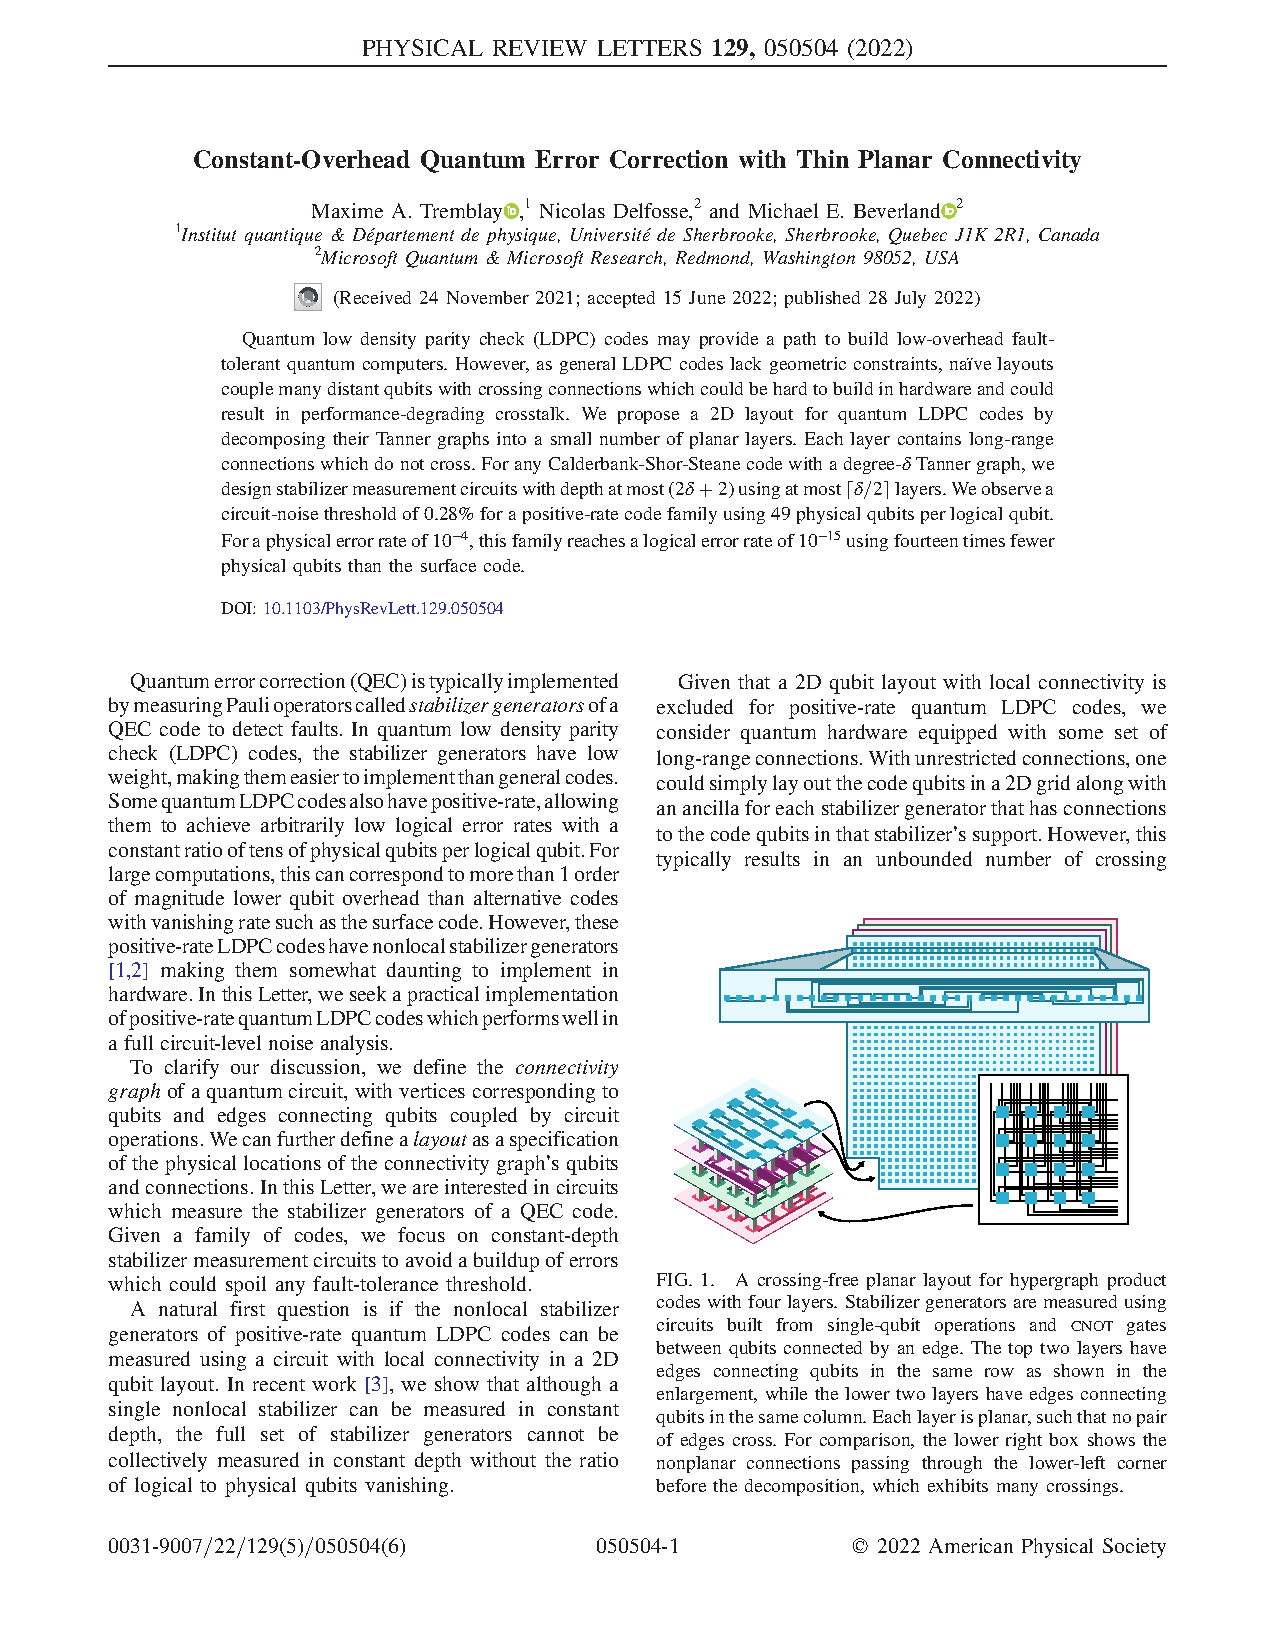
\includepdf[pages=-]{articles/planar_layout.pdf}

